\section{تولید مجموعه‌آیتم‌های مکرر}

% Slide 13: Apriori Algorithm: Basic Idea
\begin{frame}{الگوریتم آپریوری: ایدهٔ بنیادین}{\lr{Apriori Algorithm: Basic Idea}}
\begin{itemize}\setlength{\itemsep}{10pt}
    \item \textbf{رویکرد دو مرحله‌ای:} \lr{(Two-step approach)}
    \begin{enumerate}\setlength{\itemsep}{6pt}
        \item \textbf{تولید مجموعه‌آیتم‌های مکرر} \lr{(Frequent Itemset Generation)}:
        \begin{itemize}\setlength{\itemsep}{3pt}
            \item تولید تمامی مجموعه‌آیتم‌هایی که مقدار پشتیبان آن‌ها $\ge \text{minsup}$ باشد.
        \end{itemize}
        \item \textbf{تولید قواعد} \lr{(Rule Generation)}:
        \begin{itemize}\setlength{\itemsep}{3pt}
            \item تولید قواعد با اطمینان بالا از هر مجموعه‌آیتم مکرر، به‌طوری که هر قاعده یک افراز دودویی از مجموعه‌آیتم مکرر باشد.
        \end{itemize}
    \end{enumerate}
    \item \alert{\textbf{تولید مجموعه‌آیتم‌های مکرر همچنان از نظر محاسباتی بسیار سنگین و پرهزینه است!}}
\end{itemize}
\end{frame}

% Slide 14: Frequent Itemset Generation
\begin{frame}{تولید مجموعه‌آیتم‌های مکرر}{\lr{Frequent Itemset Generation}}
\begin{itemize}\setlength{\itemsep}{3pt}
    \item به ازای $d$ قلم کالا، دقیقاً \alert{$2^d$} مجموعه‌آیتم نامزد وجود دارد!
\end{itemize}
\vspace{-0.1cm}
\begin{center}
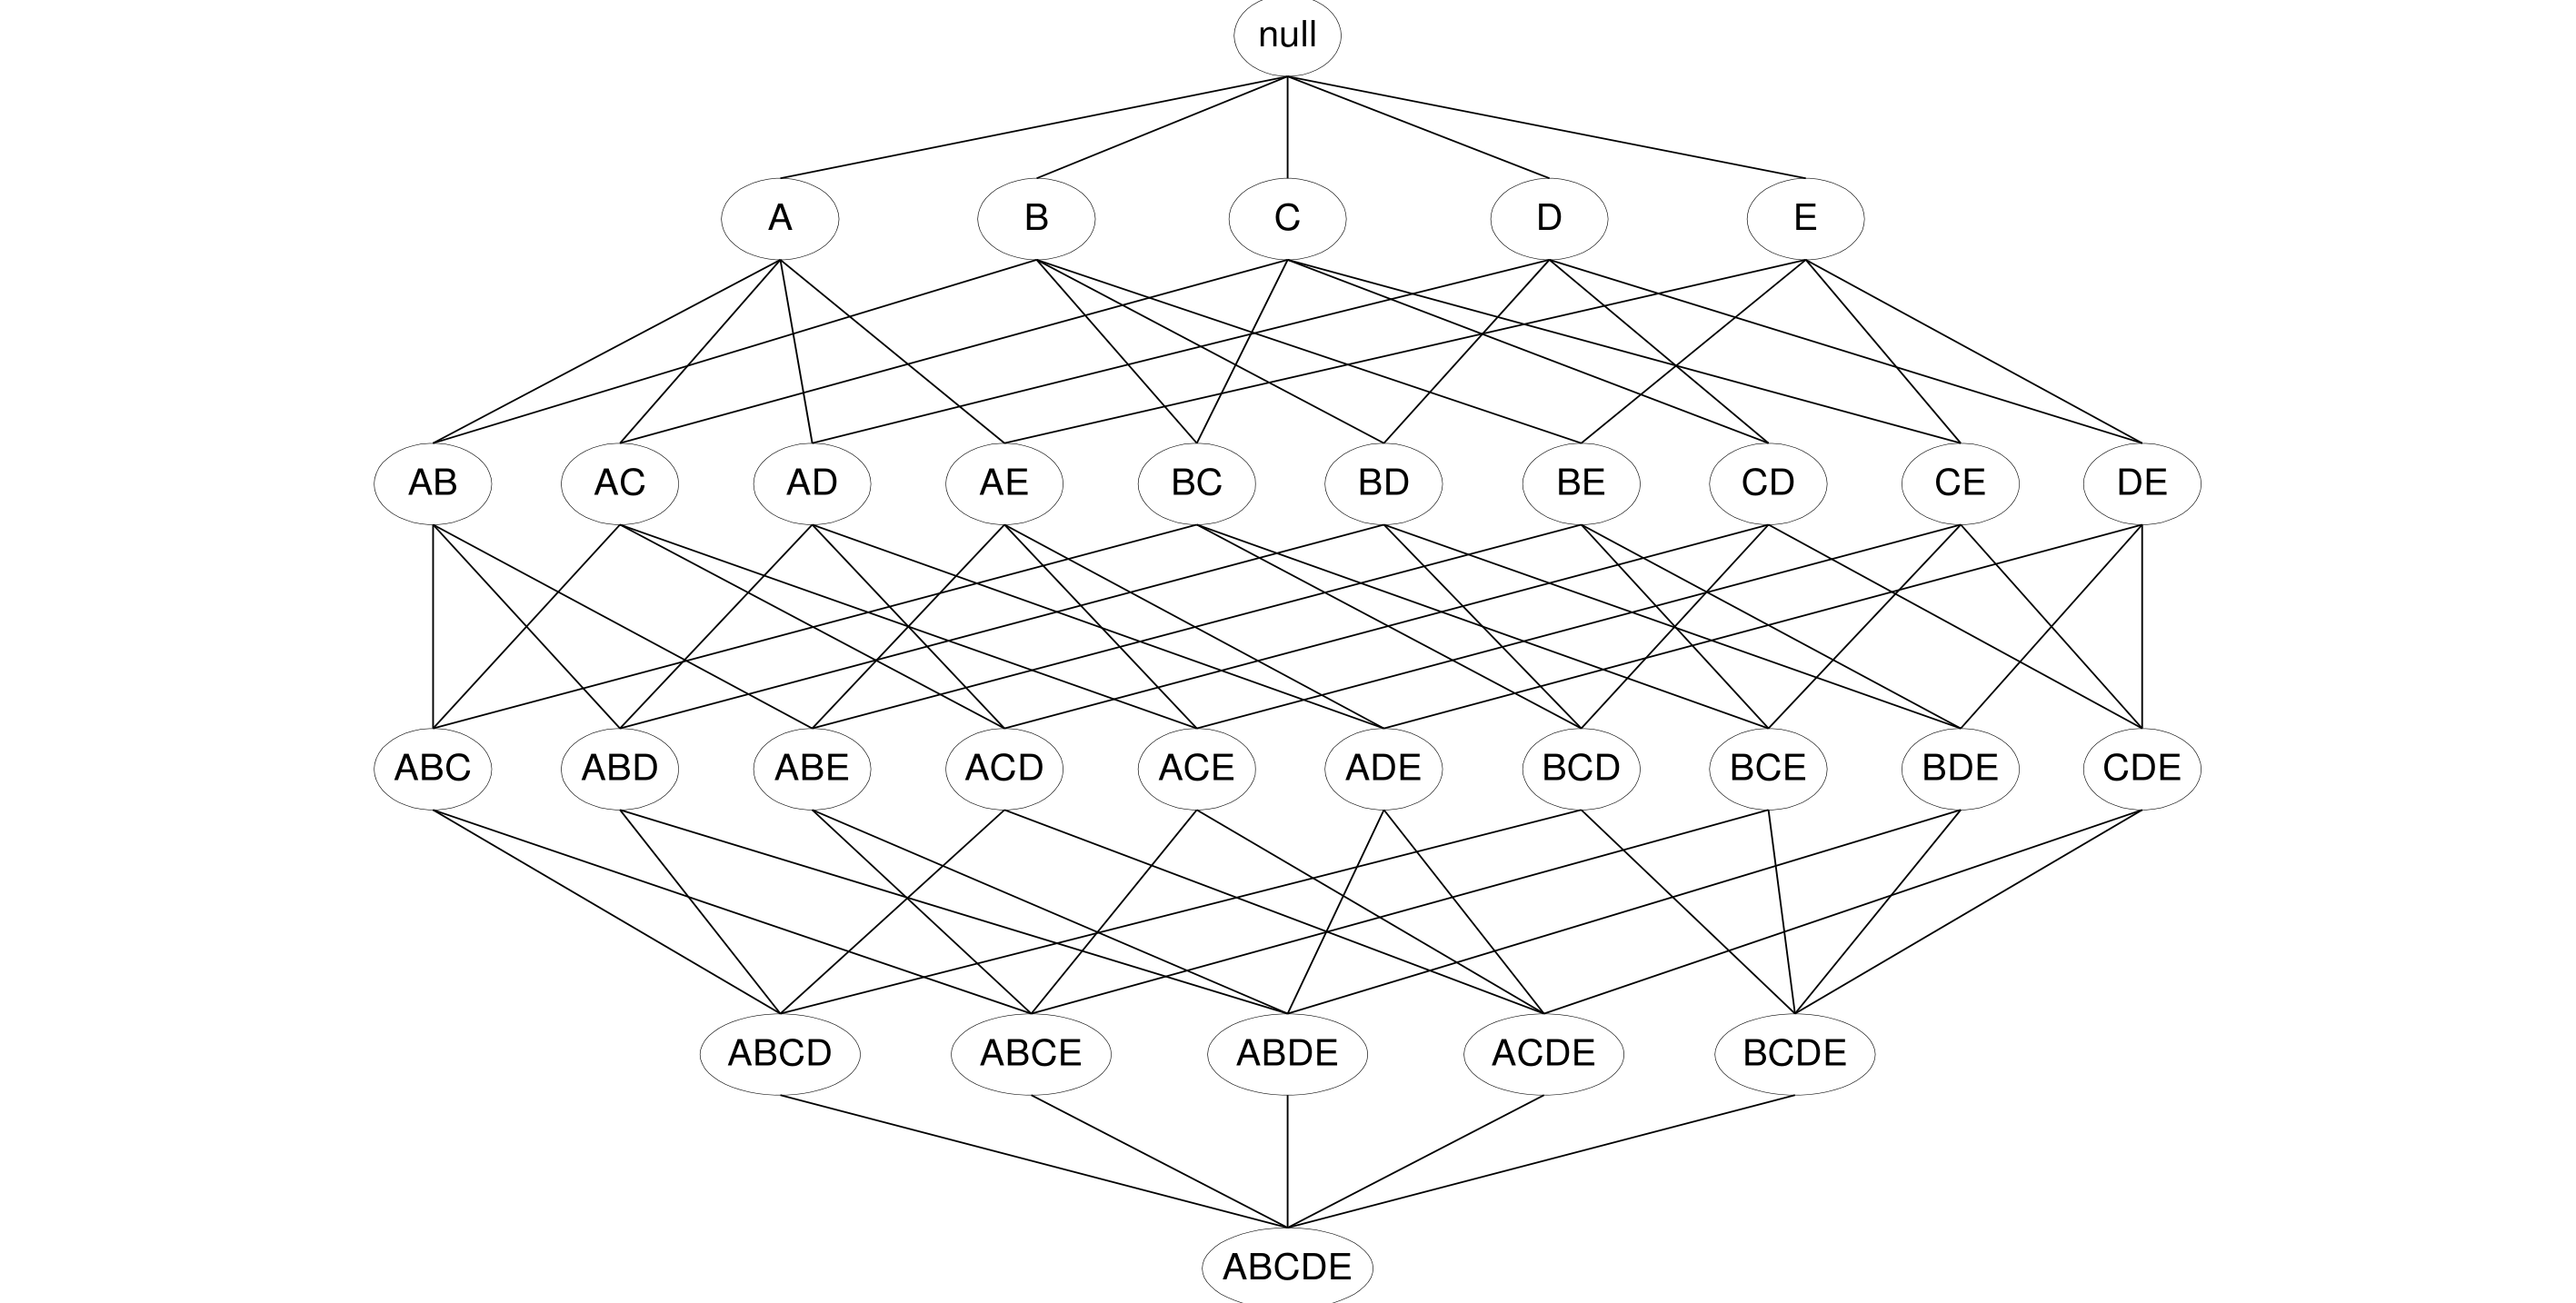
\includegraphics[width=0.82\textwidth,keepaspectratio]{images/slide14_lattice_clean.png}
\end{center}
\end{frame}

% Slide 15: Brute-force Approach
\begin{frame}{رویکرد جامع}{\lr{Brute-force Approach}}
\begin{itemize}\setlength{\itemsep}{3pt}\small
    \item هر مجموعه‌آیتم در مشبکه، یک \textbf{نامزد مکرر بودن} است.
    \item شمارش پشتیبان هر نامزد با پیمایش کل پایگاه داده انجام می‌شود.
    \item تطبیق تک‌تک تراکنش‌ها با تمام نامزدها:
\end{itemize}

\vspace{-0.15cm}
\begin{center}
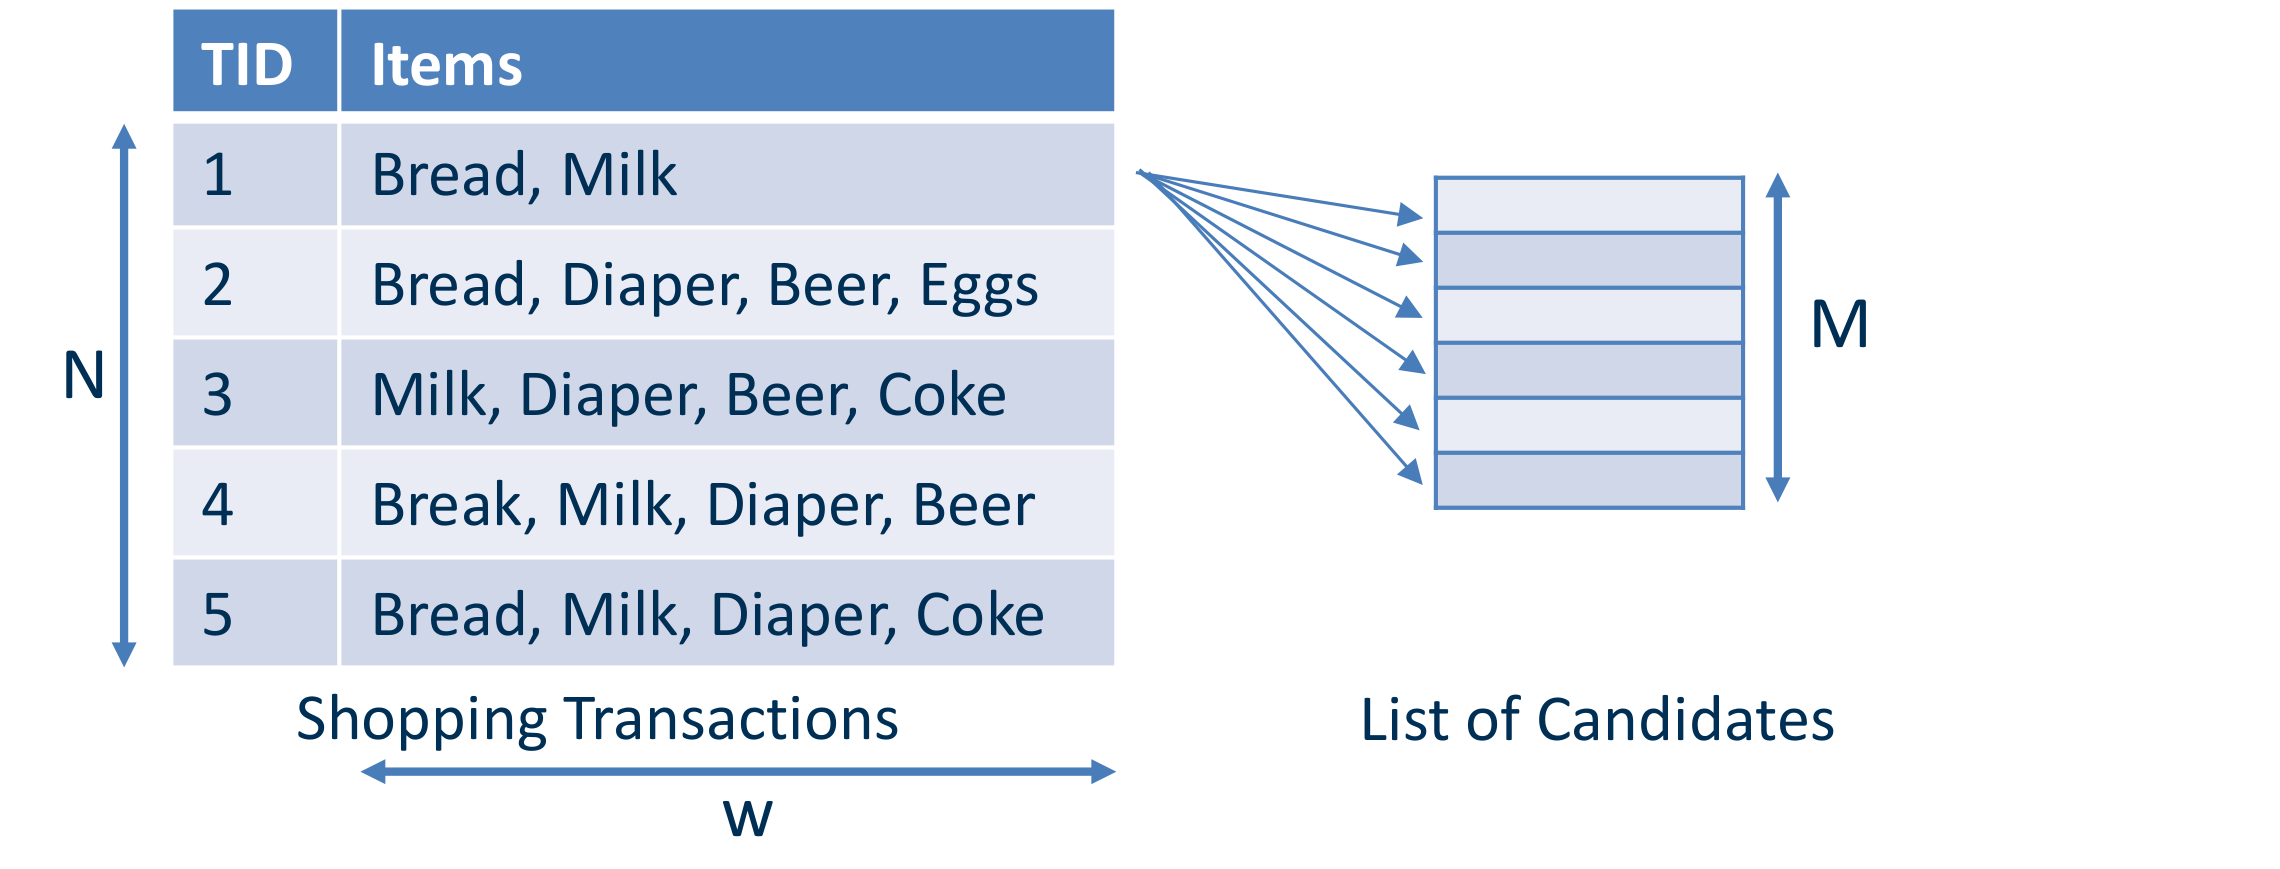
\includegraphics[width=0.82\textwidth,keepaspectratio]{images/slide15_candidates_match_clean.png}
\end{center}

\vspace{-0.15cm}
\begin{itemize}\small
    \item \textbf{پیچیدگی محاسباتی:} $\mathcal{O}(N \cdot M \cdot w)$ که در آن $M = 2^d$ است (بسیار سنگین و غیرعملی).
\end{itemize}
\end{frame}

% Slide 16: Brute-force Scale in Real-World
\begin{frame}{رویکرد جامع در مقیاس واقعی}{\lr{Brute-force Approach}}
\begin{itemize}\setlength{\itemsep}{4pt}\small
    \item \textbf{آمازون} دارای بیش از ۱۲ میلیون محصول مختلف است (تا سال \lr{2023}):
    \begin{itemize}\footnotesize
        \item یعنی $2^{12,000,000}$ مجموعه‌آیتم ممکن!
        \item عددی با \lr{3.6} میلیون رقم!
    \end{itemize}
    \item \textbf{سریع‌ترین ابررایانه‌های امروزی:} حدود ۱,۲۰۰ پتافلاپس ($1.2 \times 10^{18}$ عملیات در ثانیه).
    \item \textbf{تعداد اتم‌های جهان قابل‌مشاهده:} حدود $10^{80}$.
    \item \textbf{زمان سپری‌شده از مهبانگ (بیگ بنگ):} \lr{13.8} میلیارد سال $\approx 4.35 \times 10^{17}$ ثانیه.
\end{itemize}

\vspace{0.1cm}
\begin{columns}[T,onlytextwidth]
\begin{column}{0.30\textwidth}
\centering

\includegraphics[width=0.88\linewidth,height=1.8cm,keepaspectratio]{images/slide16_amazon.png}\\[2pt]
{\tiny\lr{12M Products}}
\end{column}%
\begin{column}{0.30\textwidth}
\centering
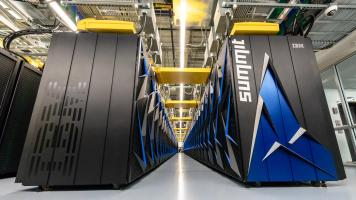
\includegraphics[width=0.88\linewidth,height=1.8cm,keepaspectratio]{images/slide16_supercomputer.jpg}\\[2pt]
{\tiny\lr{1,200 Petaflops}}
\end{column}%
\begin{column}{0.30\textwidth}
\centering
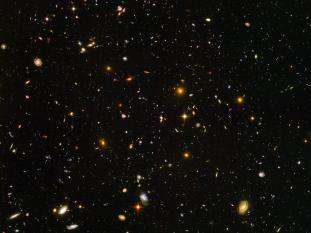
\includegraphics[width=0.88\linewidth,height=1.8cm,keepaspectratio]{images/slide16_galaxy.jpg}\\[2pt]
{\tiny\lr{Observable Universe}}
\end{column}
\end{columns}

\vspace{0.1cm}
\begin{center}
\alert{\textbf{محاسبهٔ جامع حتی از کل عمر کیهان نیز بسیار بیشتر طول می‌کشد!}}
\end{center}
\end{frame}

% Slide 17: Anti-Monotonicity of Support
\begin{frame}{خاصیت پاد‌یکنواختی پشتیبان}{\lr{Anti-Monotonicity of Support}}
\begin{columns}[T,onlytextwidth]
\begin{column}{0.58\textwidth}
\begin{itemize}\setlength{\itemsep}{5pt}
    \item \textbf{با بزرگ‌تر شدن یک مجموعه‌آیتم چه رخ می‌دهد؟}
    \begin{center}
    \begin{latin}
    \small
    $s(\{\text{Milk}\}) = 0.8$ \\
    $s(\{\text{Milk, Diaper}\}) = 0.6$ \\
    $s(\{\text{Milk, Diaper, Beer}\}) = 0.4$ \\[6pt]
    $s(\{\text{Bread}\}) = 0.8$ \\
    $s(\{\text{Bread, Milk}\}) = 0.6$ \\
    $s(\{\text{Bread, Milk, Diaper}\}) = 0.4$
    \end{latin}
    \end{center}
    \item \alert{\textbf{یک الگوی منظم و بنیادین در اینجا وجود دارد!}}
\end{itemize}
\end{column}%
\begin{column}{0.40\textwidth}
\centering
\textbf{\small تراکنش‌های خرید}\\[1pt]
{\scriptsize\lr{(Shopping Transactions)}}\\[3pt]
\begin{latin}
\fontsize{7.5}{9.5}\selectfont
\begin{tabular}{|c|l|}
\hline
\rowcolor{mannheimblue!15}
\textbf{TID} & \textbf{Items} \\ \hline
1 & {\color{teal}\textbf{Milk}}, Bread \\ \hline
2 & Bread, {\color{blue}\textbf{Diaper}}, {\color{red}\textbf{Beer}}, Eggs \\ \hline
3 & {\color{teal}\textbf{Milk}}, {\color{blue}\textbf{Diaper}}, {\color{red}\textbf{Beer}}, Coke \\ \hline
4 & Bread, {\color{teal}\textbf{Milk}}, {\color{blue}\textbf{Diaper}}, {\color{red}\textbf{Beer}} \\ \hline
5 & Bread, {\color{teal}\textbf{Milk}}, {\color{blue}\textbf{Diaper}}, Coke \\ \hline
\end{tabular}
\end{latin}
\end{column}
\end{columns}
\end{frame}

% Slide 18: Reducing the Number of Candidates
\begin{frame}{کاهش تعداد نامزدها با ویژگی پاد‌یکنواخت}{\lr{Reducing the Number of Candidates}}
\begin{itemize}\setlength{\itemsep}{6pt}
    \item \textbf{الگوی بنیادین:} خاصیت پاد‌یکنواختی پشتیبان \lr{(Anti-Monotonicity)}:
    \begin{itemize}\setlength{\itemsep}{3pt}
        \item اگر $X$ زیرمجموعه‌ای از $Y$ باشد، پشتیبان $Y$ حداکثر می‌تواند به بزرگی پشتیبان $X$ باشد:
        \begin{latin}
        \[
        \forall X, Y: \quad X \subseteq Y \implies s(X) \ge s(Y)
        \]
        \end{latin}
    \end{itemize}
    \item \textbf{پیامدها و هرس:}
    \begin{itemize}\setlength{\itemsep}{3pt}
        \item اگر یک مجموعه‌آیتم \textbf{مکرر} باشد، تمام زیرمجموعه‌های آن نیز قطعاً مکرر هستند.
        \item \alert{\textbf{اصل آپریوری (قاعدهٔ هرس):}} اگر یک مجموعه‌آیتم \textbf{نامکرر} باشد، تمام ابرمجموعه‌های آن نیز قطعاً \textbf{نامکرر} خواهند بود و نیازی به بررسی آن‌ها نیست!
    \end{itemize}
\end{itemize}
\end{frame}

% Slide 19: Using Apriori Principle for Pruning
\begin{frame}{هرس فضای جستجو بر اساس اصل آپریوری}{\lr{Using the Apriori Principle for Pruning}}
\begin{center}
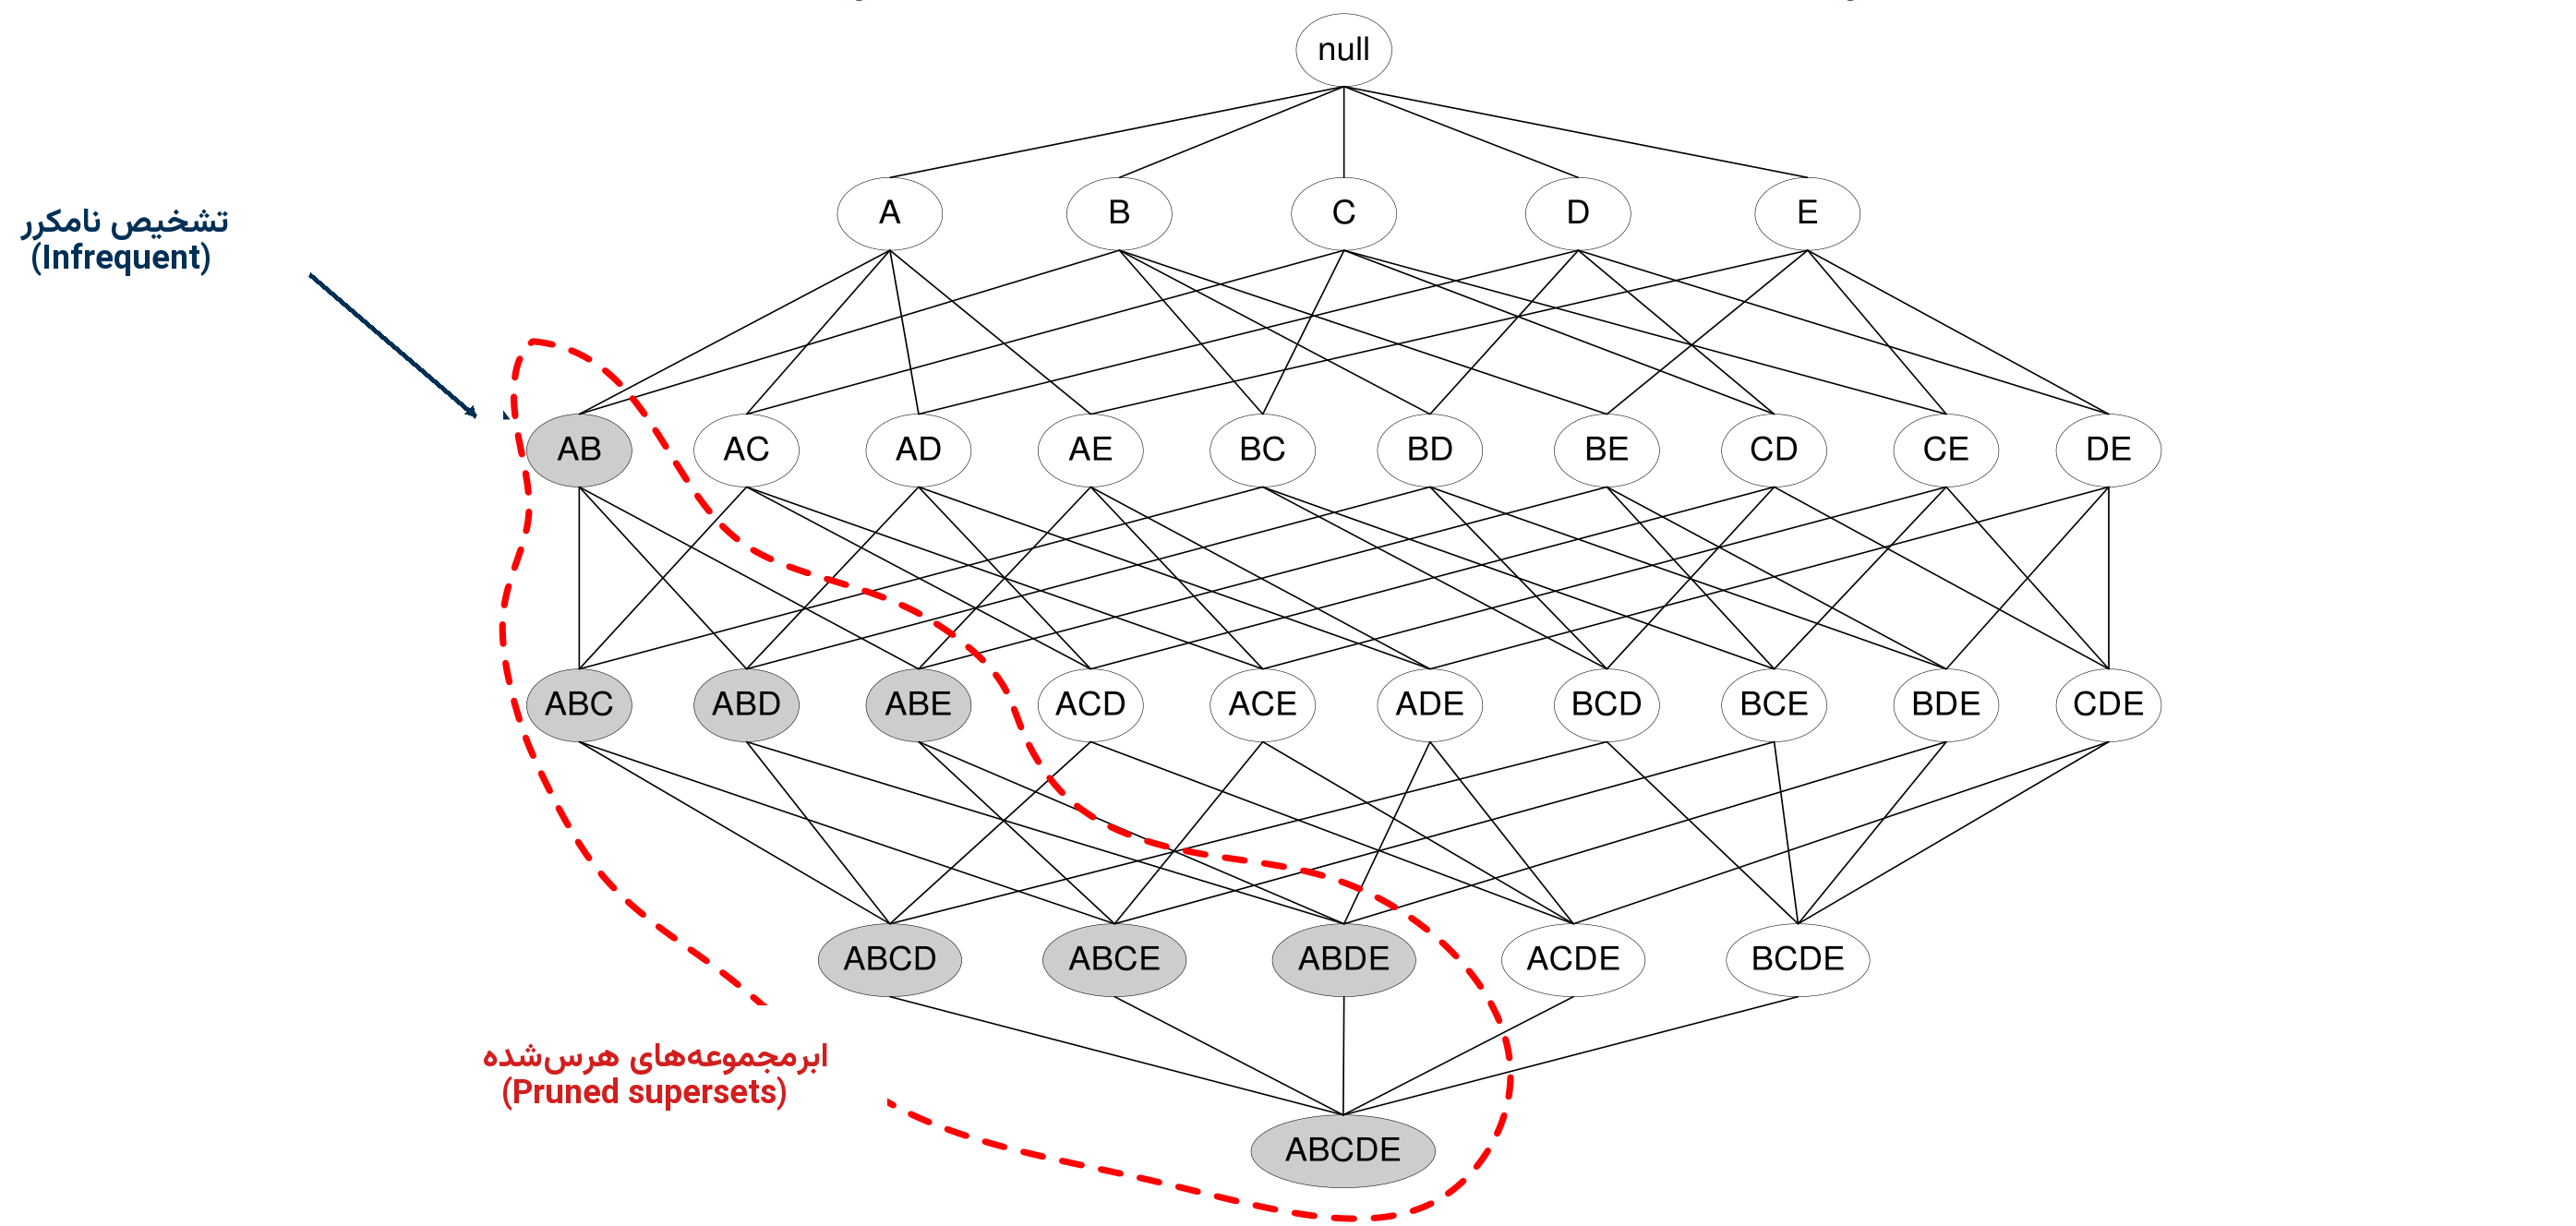
\includegraphics[width=0.88\textwidth,keepaspectratio]{images/slide19_pruning_perfect.png}
\end{center}
\vspace{-0.2cm}
\begin{center}
\small اگر یک مجموعه‌آیتم نامکرر باشد، تمام ابرمجموعه‌های آن فوراً هرس می‌شوند.
\end{center}
\end{frame}

% Slide 20: The Apriori Algorithm
\begin{frame}{الگوریتم آپریوری}{\lr{The Apriori Algorithm}}
\begin{itemize}\setlength{\itemsep}{7pt}
    \item مقدار $k=1$ قرار داده می‌شود.
    \item مجموعه‌آیتم‌های مکرر به طول ۱ ($F_1$) تولید می‌شوند.
    \item \textbf{تکرار تا زمانی که هیچ مجموعه‌آیتم مکرر جدیدی شناسایی نشود:}
    \begin{itemize}\setlength{\itemsep}{4pt}
        \item \textbf{تولید نامزدها:} تولید مجموعه‌آیتم‌های نامزد به طول $k+1$ از روی اقلام مکرر به طول $k$.
        \item \textbf{هرس نامزدها:} هرس نامزدهایی که شامل زیرمجموعه‌ای نامکرر به طول $k$ هستند (بر اساس اصل آپریوری).
        \item \textbf{شمارش پشتیبان:} شمارش پشتیبان هر نامزد با پیمایش پایگاه داده.
        \item \textbf{حذف نامکررها:} حذف نامزدهای نامکرر، و نگه‌داشتن موارد مکرر ($F_{k+1}$).
        \item $k = k + 1$
    \end{itemize}
\end{itemize}
\end{frame}

% Slide 21: Illustrating Apriori Principle
\begin{frame}{تشریح اصل آپریوری با مثال عددی}{\lr{Illustrating the Apriori Principle}}
\begin{columns}[T,onlytextwidth]
\begin{column}{0.60\textwidth}
\textbf{\footnotesize حداقل شمارش پشتیبان: $\text{minsup} = 3$}\\[3pt]
\begin{minipage}{0.46\linewidth}
\textbf{\scriptsize مجموعه‌آیتم‌های ۱-عضوی:}\\[1pt]
\begin{latin}
\fontsize{7}{8.5}\selectfont
\begin{tabular}{|l|c|}
\hline
\rowcolor{mannheimblue!15}\textbf{Item} & \textbf{Count} \\ \hline
Bread & 4 \\ \hline
\rowcolor{black!15}Coke & 2 \\ \hline
Milk & 4 \\ \hline
Beer & 3 \\ \hline
Diaper & 4 \\ \hline
\rowcolor{black!15}Eggs & 1 \\ \hline
\end{tabular}
\end{latin}
\end{minipage}\hfill
\begin{minipage}{0.50\linewidth}
\begin{tcolorbox}[colback=orange!10,colframe=orange!80!black,arc=2pt,left=2pt,right=2pt,top=2pt,bottom=2pt]
\centering
\scriptsize بدون نیاز به تولید نامزدهای شامل \lr{Coke} یا \lr{Eggs}!
\end{tcolorbox}
\end{minipage}

\vspace{0.15cm}
\textbf{\scriptsize مجموعه‌آیتم‌های ۲-عضوی و ۳-عضوی:}\\[1pt]
\begin{minipage}{0.49\linewidth}
\begin{latin}
\fontsize{6.5}{7.5}\selectfont
\begin{tabular}{|l|c|}
\hline
\rowcolor{mannheimblue!15}\textbf{2-pairs} & \textbf{Count} \\ \hline
\{Bread, Milk\} & 3 \\ \hline
\rowcolor{black!15}\{Bread, Beer\} & 2 \\ \hline
\{Bread, Diaper\} & 3 \\ \hline
\rowcolor{black!15}\{Milk, Beer\} & 2 \\ \hline
\{Milk, Diaper\} & 3 \\ \hline
\{Beer, Diaper\} & 3 \\ \hline
\end{tabular}
\end{latin}
\end{minipage}\hfill
\begin{minipage}{0.49\linewidth}
\begin{latin}
\fontsize{6.5}{7.5}\selectfont
\begin{tabular}{|l|c|}
\hline
\rowcolor{mannheimblue!15}\textbf{3-itemset} & \textbf{Count} \\ \hline
\{Bread, Milk, Diaper\} & 3 \\ \hline
\end{tabular}
\end{latin}
\vspace{0.1cm}
{\scriptsize عدم تولید \lr{\{Milk, Diaper, Beer\}} به دلیل نامکرر بودن \lr{\{Milk, Beer\}}.}
\end{minipage}

\end{column}%
\begin{column}{0.38\textwidth}
\centering
\textbf{\small تراکنش‌های خرید}\\[1pt]
{\scriptsize\lr{(Shopping Transactions)}}\\[3pt]
\begin{latin}
\fontsize{7.5}{9.5}\selectfont
\begin{tabular}{|c|l|}
\hline
\rowcolor{mannheimblue!15}
\textbf{TID} & \textbf{Items} \\ \hline
1 & Bread, Milk \\ \hline
2 & Bread, Diaper, Beer, Eggs \\ \hline
3 & Milk, Diaper, Beer, Coke \\ \hline
4 & Bread, Milk, Diaper, Beer \\ \hline
5 & Bread, Milk, Diaper, Coke \\ \hline
\end{tabular}
\end{latin}
\end{column}
\end{columns}
\end{frame}

% Slide 22: Illustrating Apriori Principle Summary
\begin{frame}{تشریح اصل آپریوری با مثال عددی}{\lr{Illustrating the Apriori Principle}}
\begin{columns}[T,onlytextwidth]
\begin{column}{0.58\textwidth}
\begin{itemize}\setlength{\itemsep}{6pt}
    \item در این مثال با ۶ قلم کالا، الگوریتم آپریوری تنها موارد زیر را بررسی نمود:
    \begin{itemize}\setlength{\itemsep}{3pt}
        \item ۶ مورد از مجموعه‌آیتم‌های ۱-عضوی
        \item ۶ مورد از مجموعه‌آیتم‌های ۲-عضوی
        \item ۱ مورد از مجموعه‌آیتم‌های ۳-عضوی
        \item \textbf{در مجموع تنها ۱۳ مجموعه‌آیتم بررسی شد!}
    \end{itemize}
    \vspace{0.2cm}
    \item \alert{\textbf{در مقایسه با تمام مجموعه‌آیتم‌های ممکن:}}
    \[
    2^6 = 64
    \]
    \item \textbf{نتیجه:} کاهش چشمگیر و صرفه‌جویی نزدیک به ۸۰٪ در فضای جستجو!
\end{itemize}
\end{column}%
\begin{column}{0.40\textwidth}
\centering
\textbf{\small تراکنش‌های خرید}\\[2pt]
\begin{latin}
\fontsize{7.5}{9.5}\selectfont
\begin{tabular}{|c|l|}
\hline
\rowcolor{mannheimblue!15}
\textbf{TID} & \textbf{Items} \\ \hline
1 & Bread, Milk \\ \hline
2 & Bread, Diaper, Beer, Eggs \\ \hline
3 & Milk, Diaper, Beer, Coke \\ \hline
4 & Bread, Milk, Diaper, Beer \\ \hline
5 & Bread, Milk, Diaper, Coke \\ \hline
\end{tabular}
\end{latin}

\vspace{0.3cm}
\textbf{\small شمارش مجموعه‌آیتم‌های ۱-عضوی:}\\[2pt]
\begin{latin}
\fontsize{7.5}{9.5}\selectfont
\begin{tabular}{|l|c|}
\hline
\rowcolor{mannheimblue!15}\textbf{Item} & \textbf{Count} \\ \hline
Bread & 4 \\ \hline
\rowcolor{black!15}Coke & 2 \\ \hline
Milk & 4 \\ \hline
Beer & 3 \\ \hline
Diaper & 4 \\ \hline
\rowcolor{black!15}Eggs & 1 \\ \hline
\end{tabular}
\end{latin}
\end{column}
\end{columns}
\end{frame}
